% Copyright (c)  2019  FSC.
% Permission is granted to copy, distribute and/or modify this document
% under the terms of the GNU Free Documentation License, Version 1.3
% or any later version published by the Free Software Foundation;
% with no Invariant Sections, no Front-Cover Texts, and no Back-Cover Texts.
% A copy of the license is included in the section entitled "GNU
% Free Documentation License".

\begin{figure}[H]
	\centering
	\caption{Prototipo di comunicazione: landing page.}
	\label{fig:prototipo-comunicazione:landing-page}
	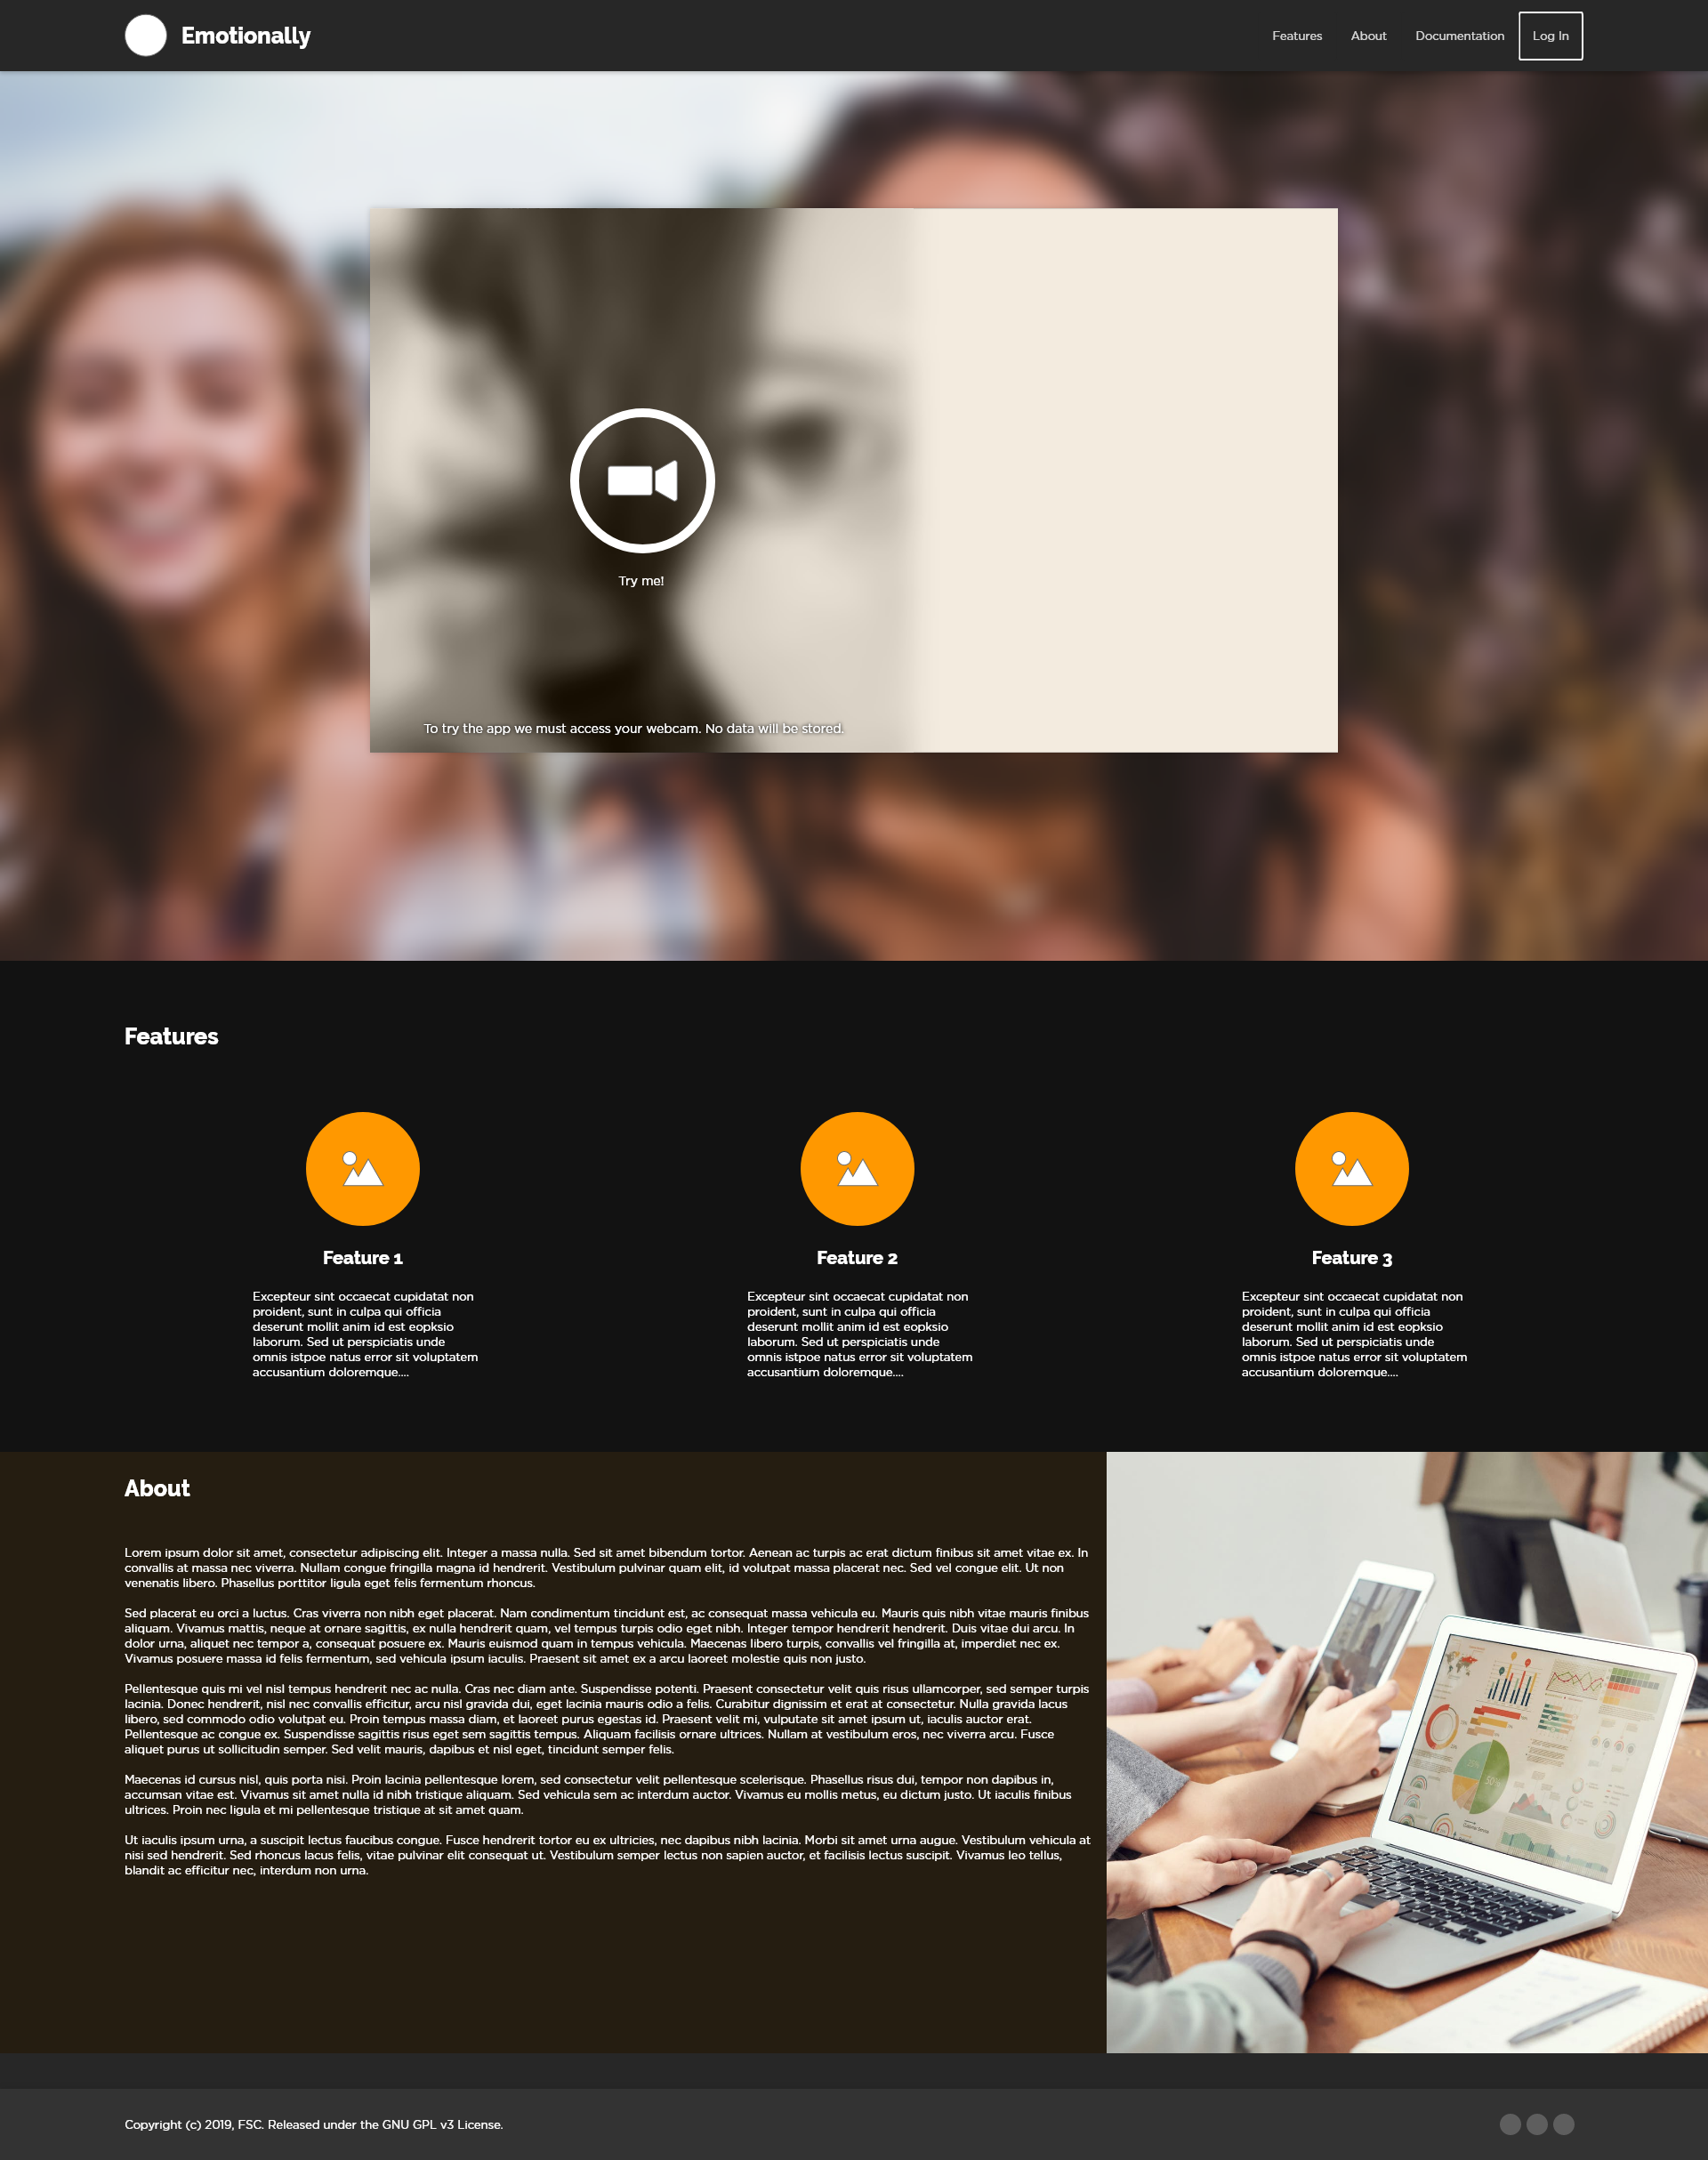
\includegraphics[width=\textwidth]{images/prototipo-comunicazione/Landing.png}
\end{figure}

\begin{figure}[H]
	\centering
	\caption{Prototipo di comunicazione: pagina di login (1).}
	\label{fig:prototipo-comunicazione:login-1}
	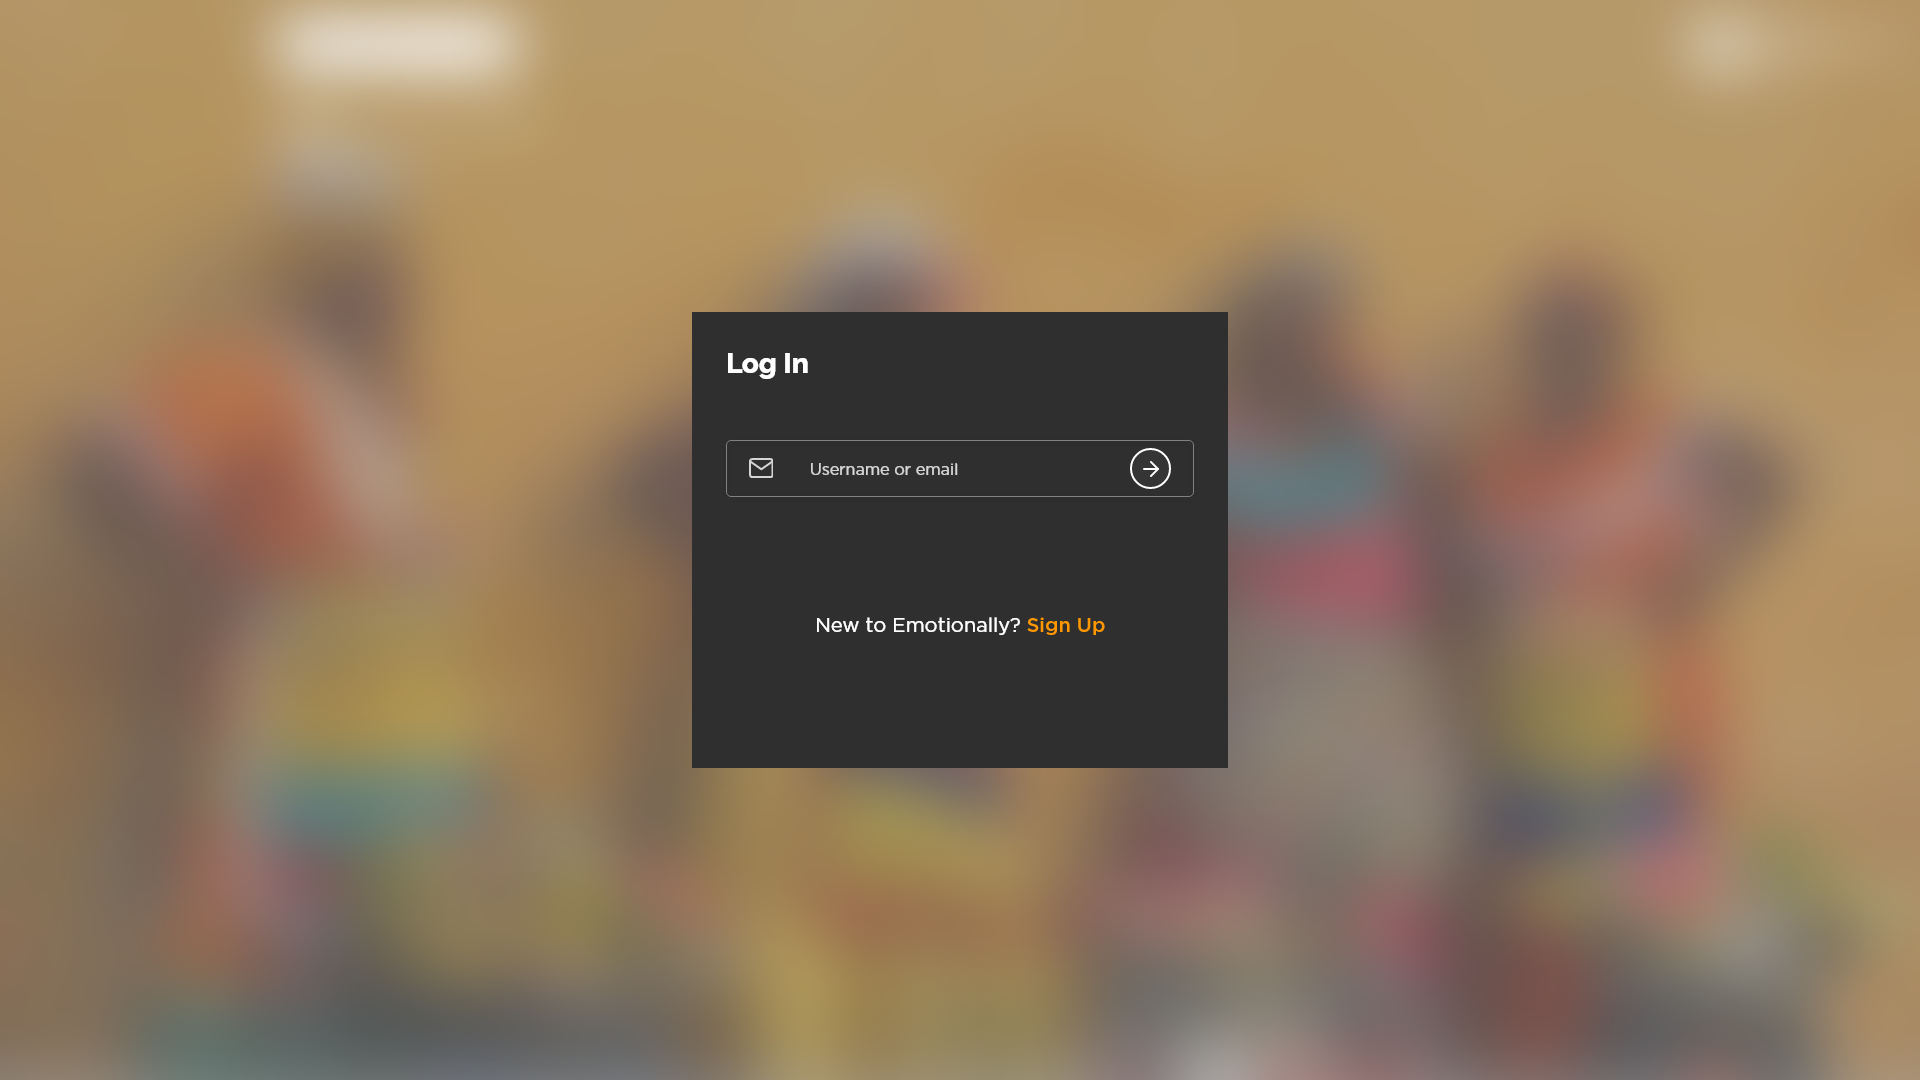
\includegraphics[width=\textwidth]{images/prototipo-comunicazione/login-1.png}
\end{figure}

\begin{figure}[H]
	\centering
	\caption{Prototipo di comunicazione: pagina di login (2).}
	\label{fig:prototipo-comunicazione:login-2}
	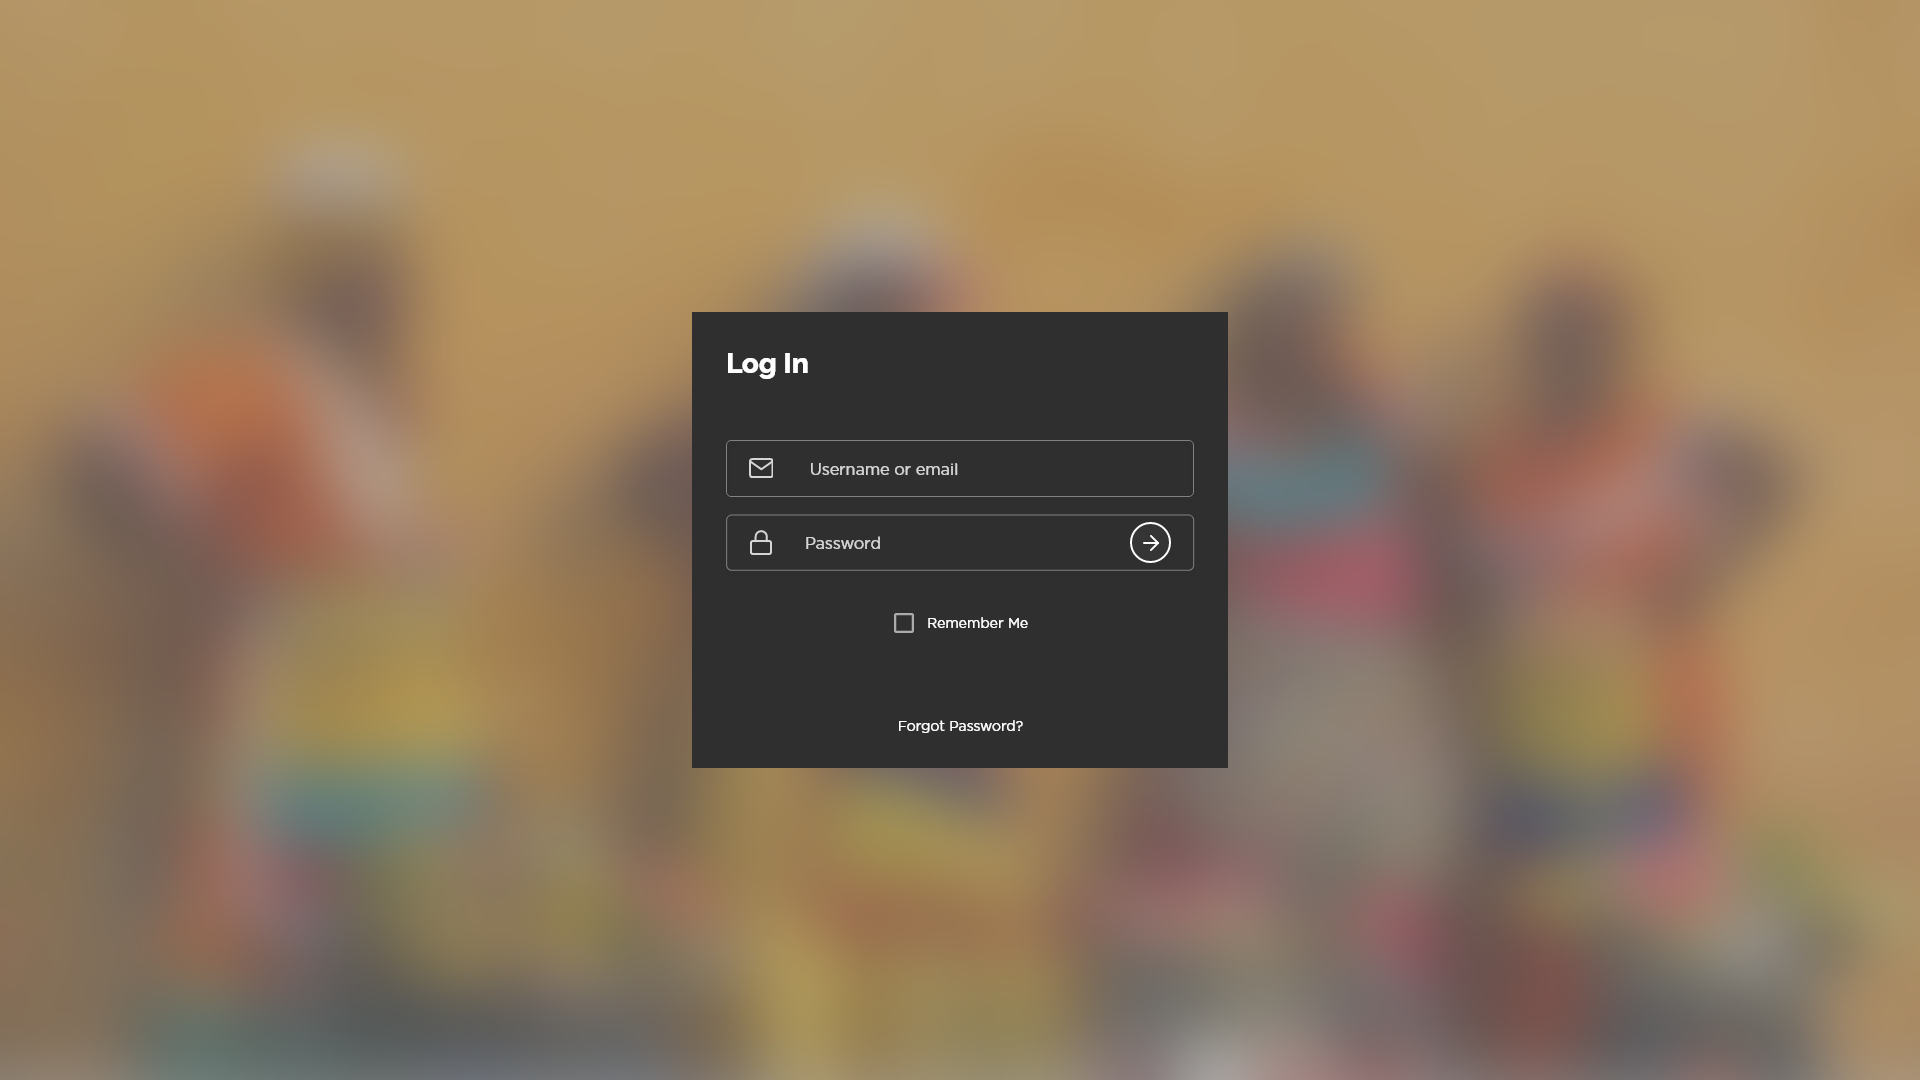
\includegraphics[width=\textwidth]{images/prototipo-comunicazione/login-2.png}
\end{figure}

\begin{figure}[H]
	\centering
	\caption{Prototipo di comunicazione: pagina di registrazione.}
	\label{fig:prototipo-comunicazione:registrazione}
	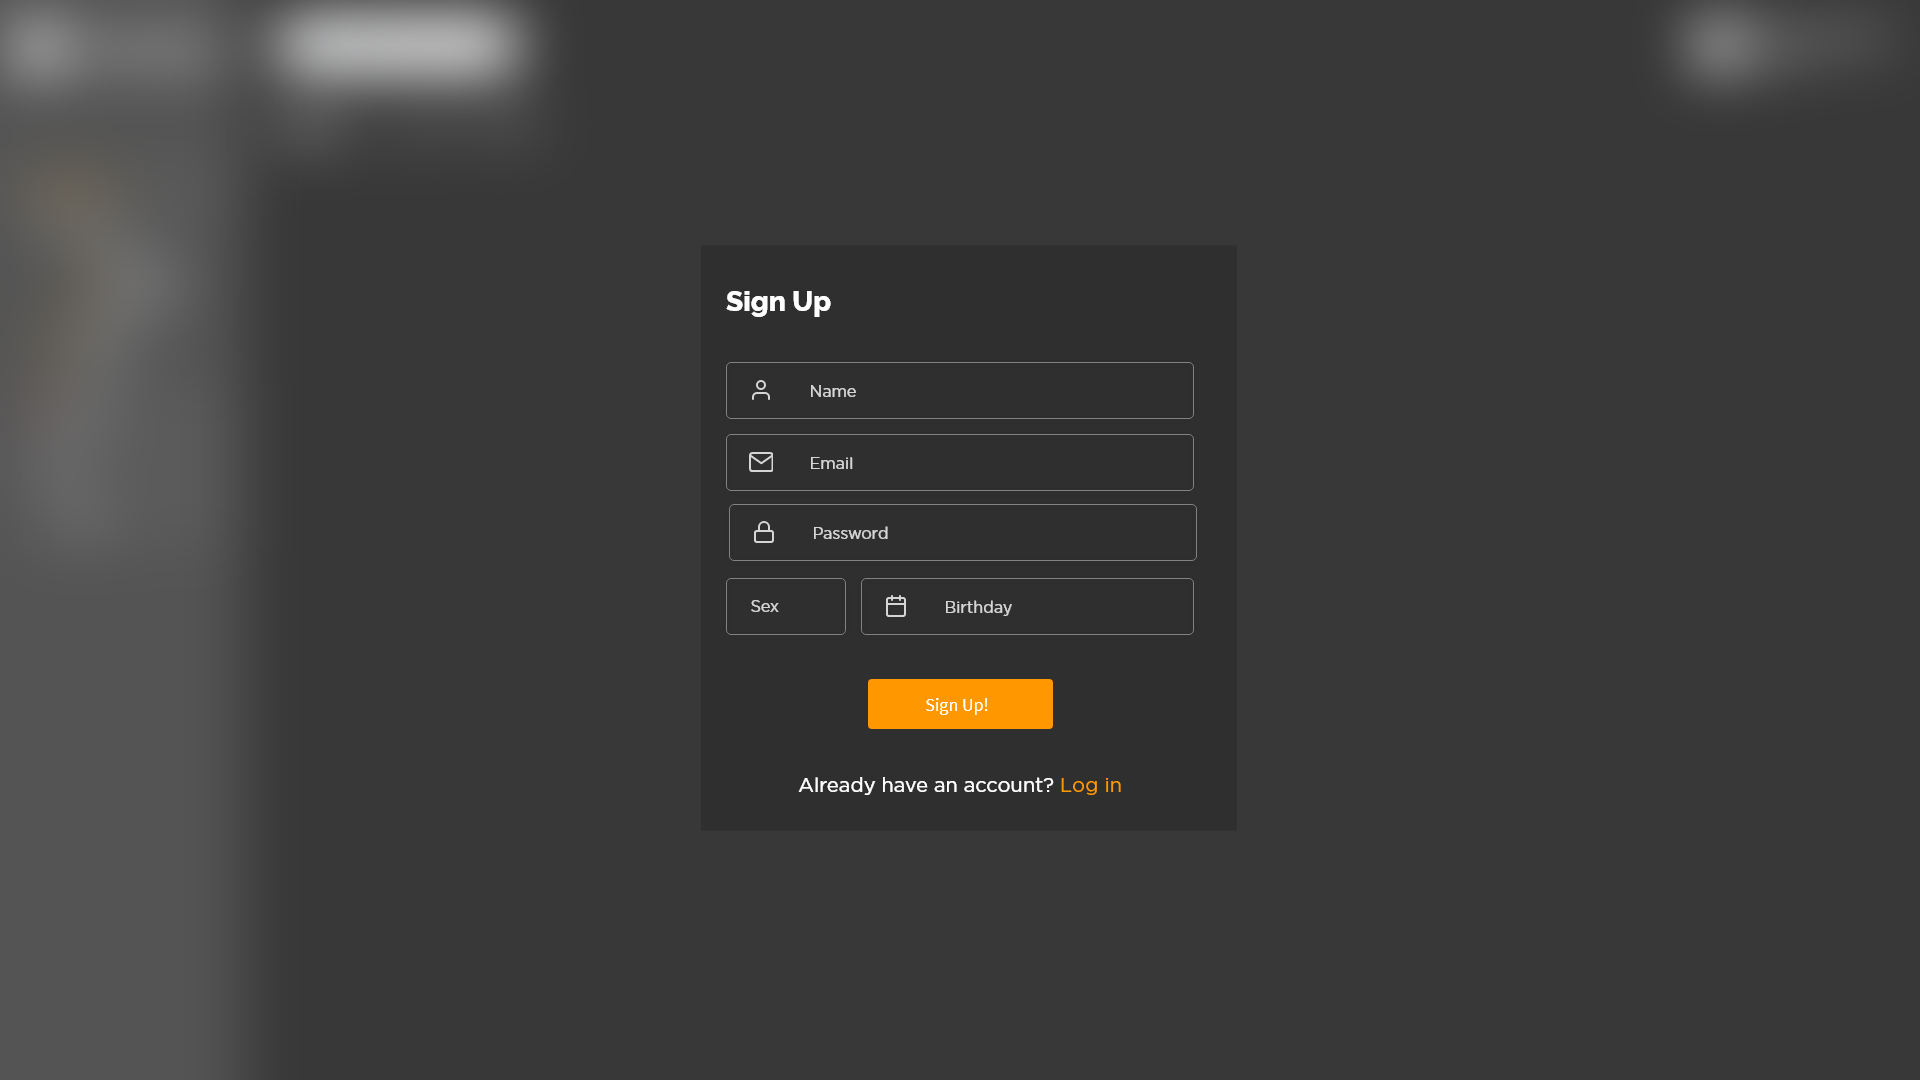
\includegraphics[width=\textwidth]{images/prototipo-comunicazione/registrazione.png}
\end{figure}

\begin{figure}[H]
	\centering
	\caption{Prototipo di comunicazione: pagina home.}
	\label{fig:prototipo-comunicazione:home}
	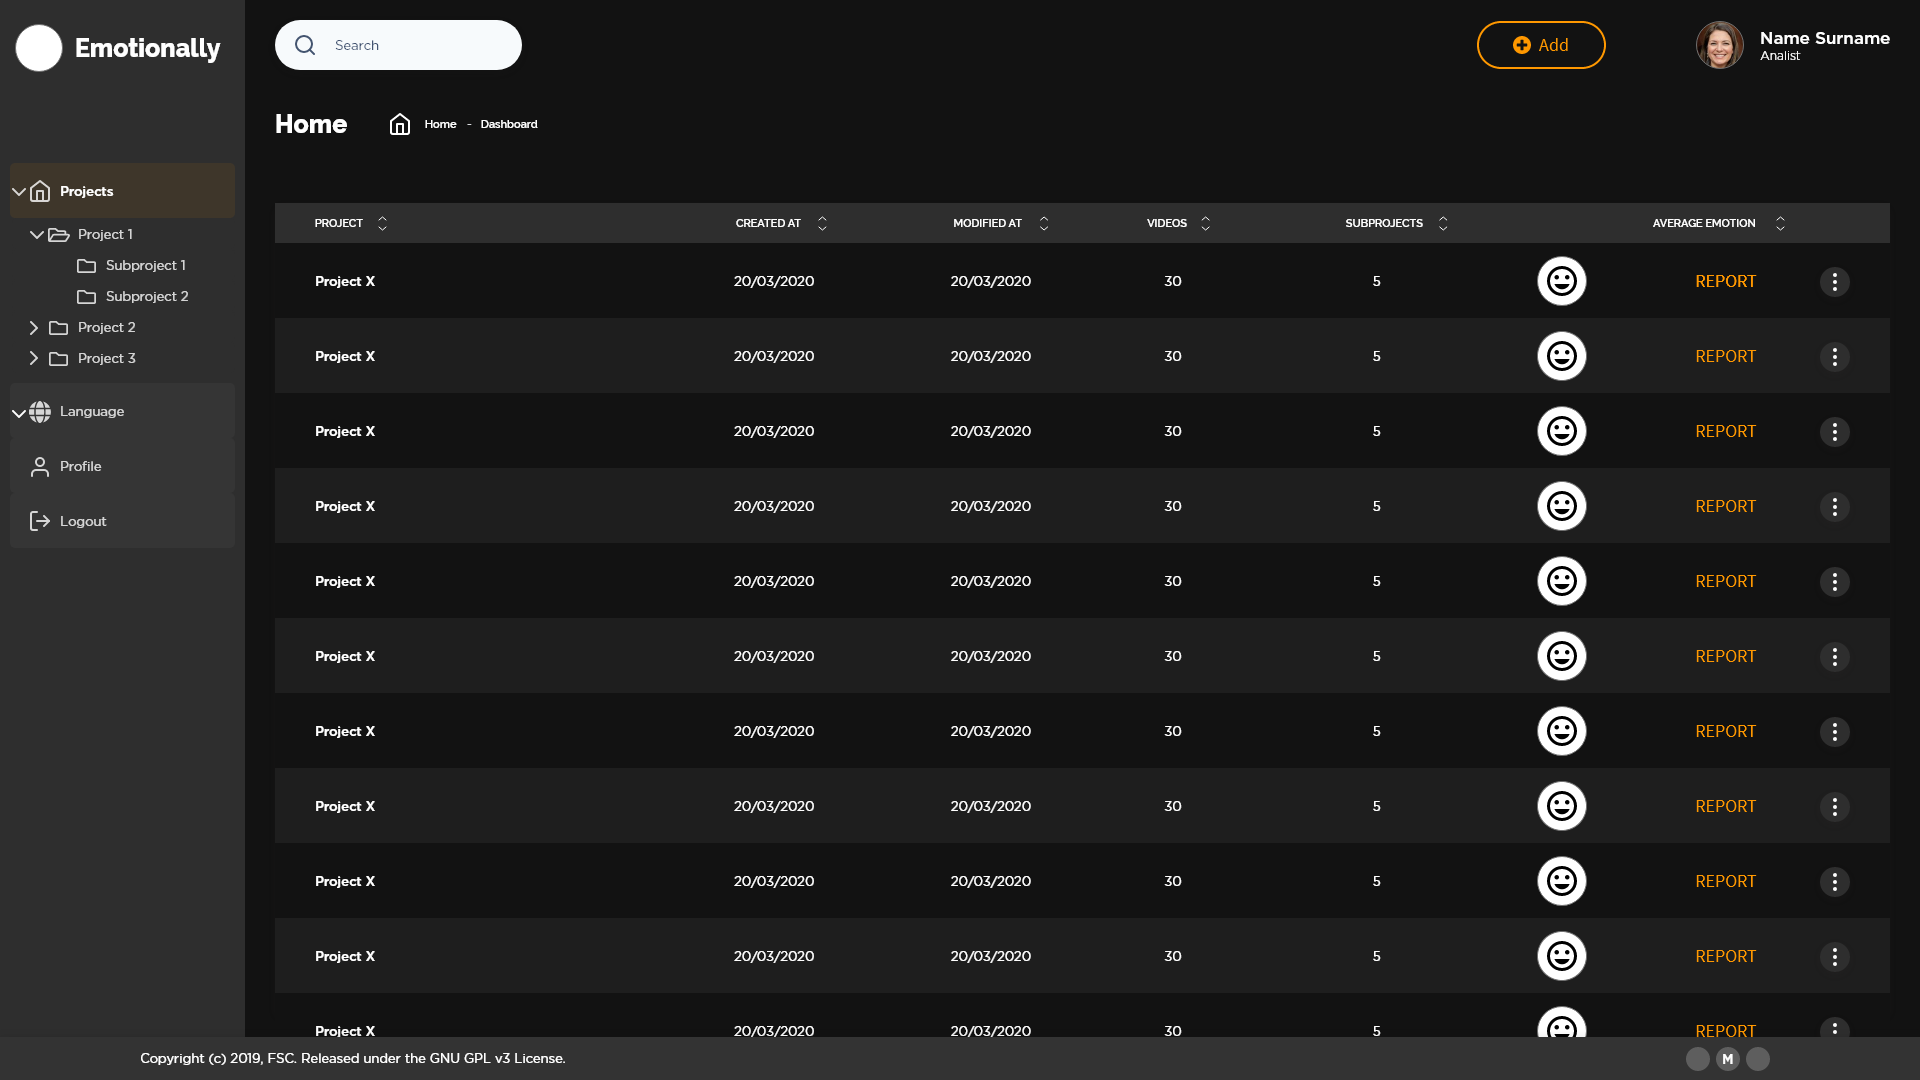
\includegraphics[width=\textwidth]{images/prototipo-comunicazione/home-no-scroll.png}
\end{figure}

\begin{figure}[H]
	\centering
	\caption{Prototipo di comunicazione: pagina di un progetto.}
	\label{fig:prototipo-comunicazione:project}
	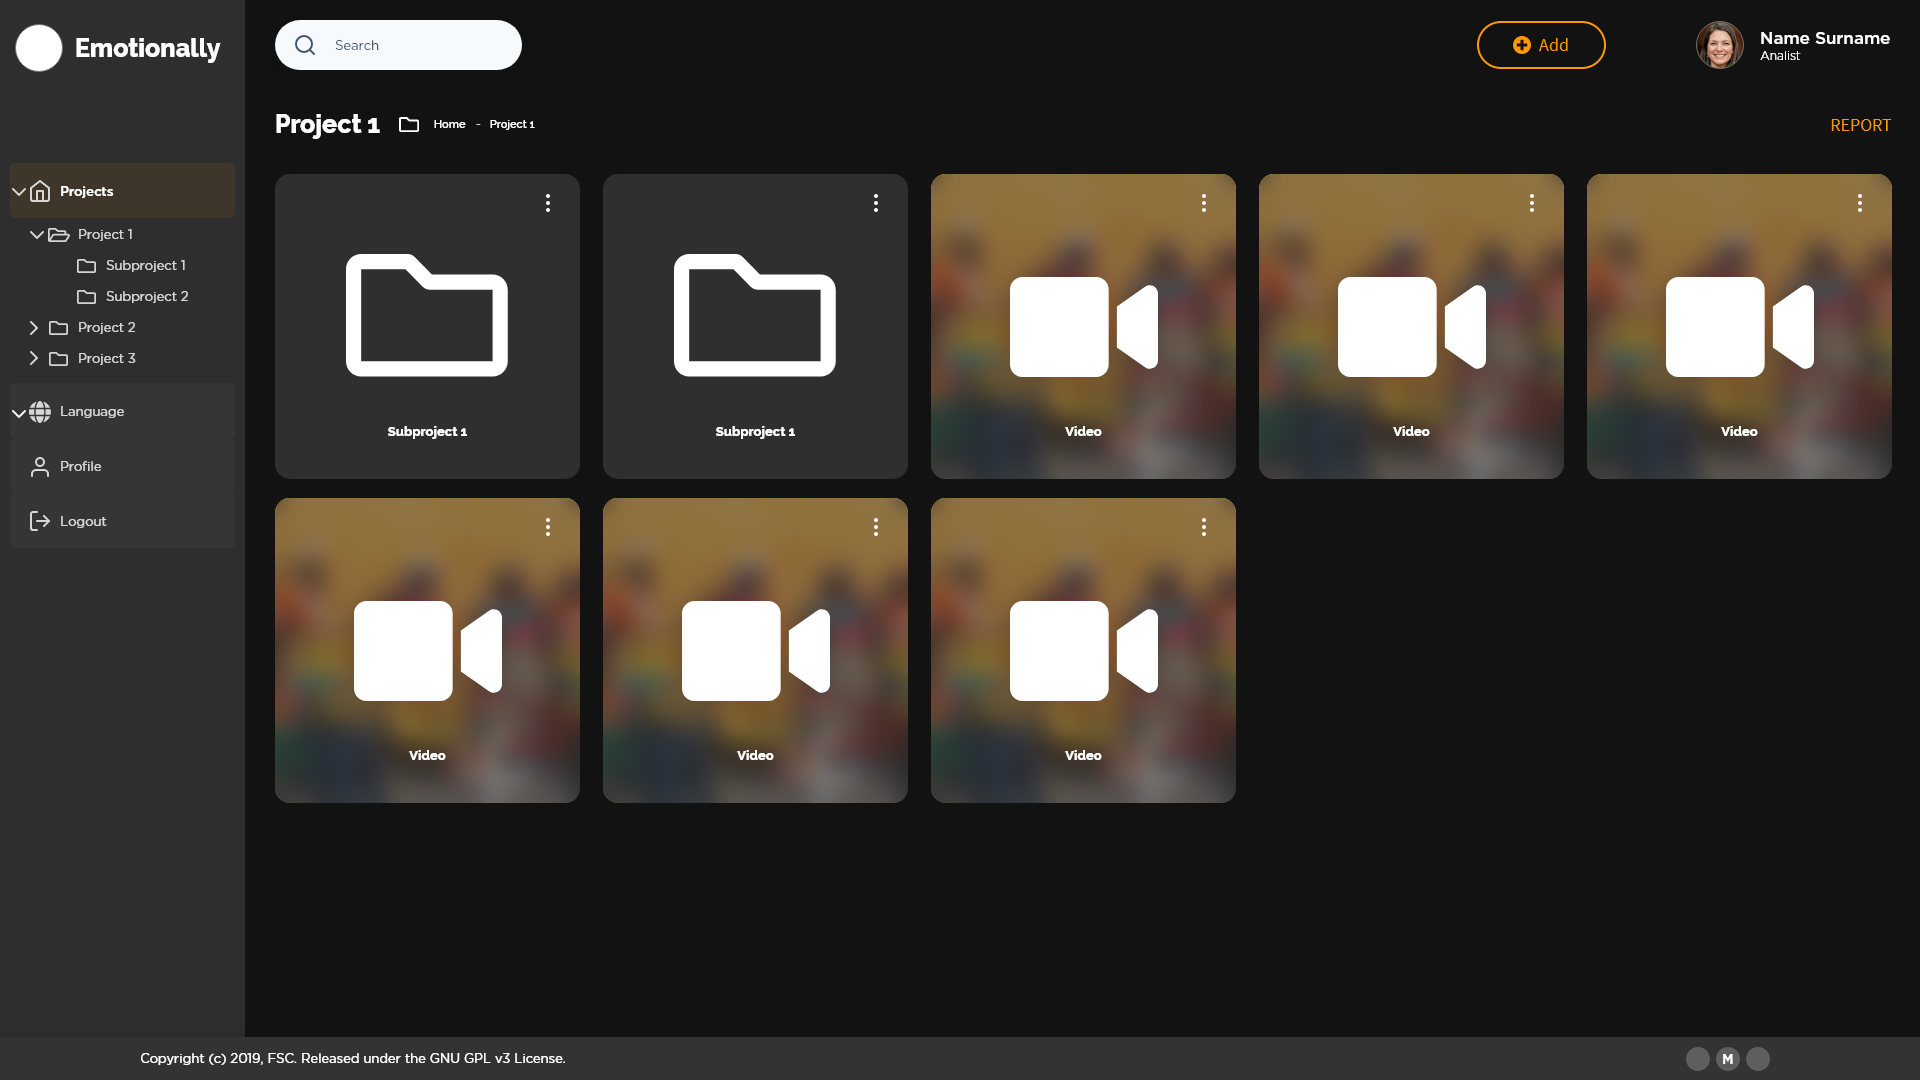
\includegraphics[width=\textwidth]{images/prototipo-comunicazione/project.png}
\end{figure}

\begin{figure}[H]
	\centering
	\caption{Prototipo di comunicazione: pagina di un sottoprogetto.}
	\label{fig:prototipo-comunicazione:subproject}
	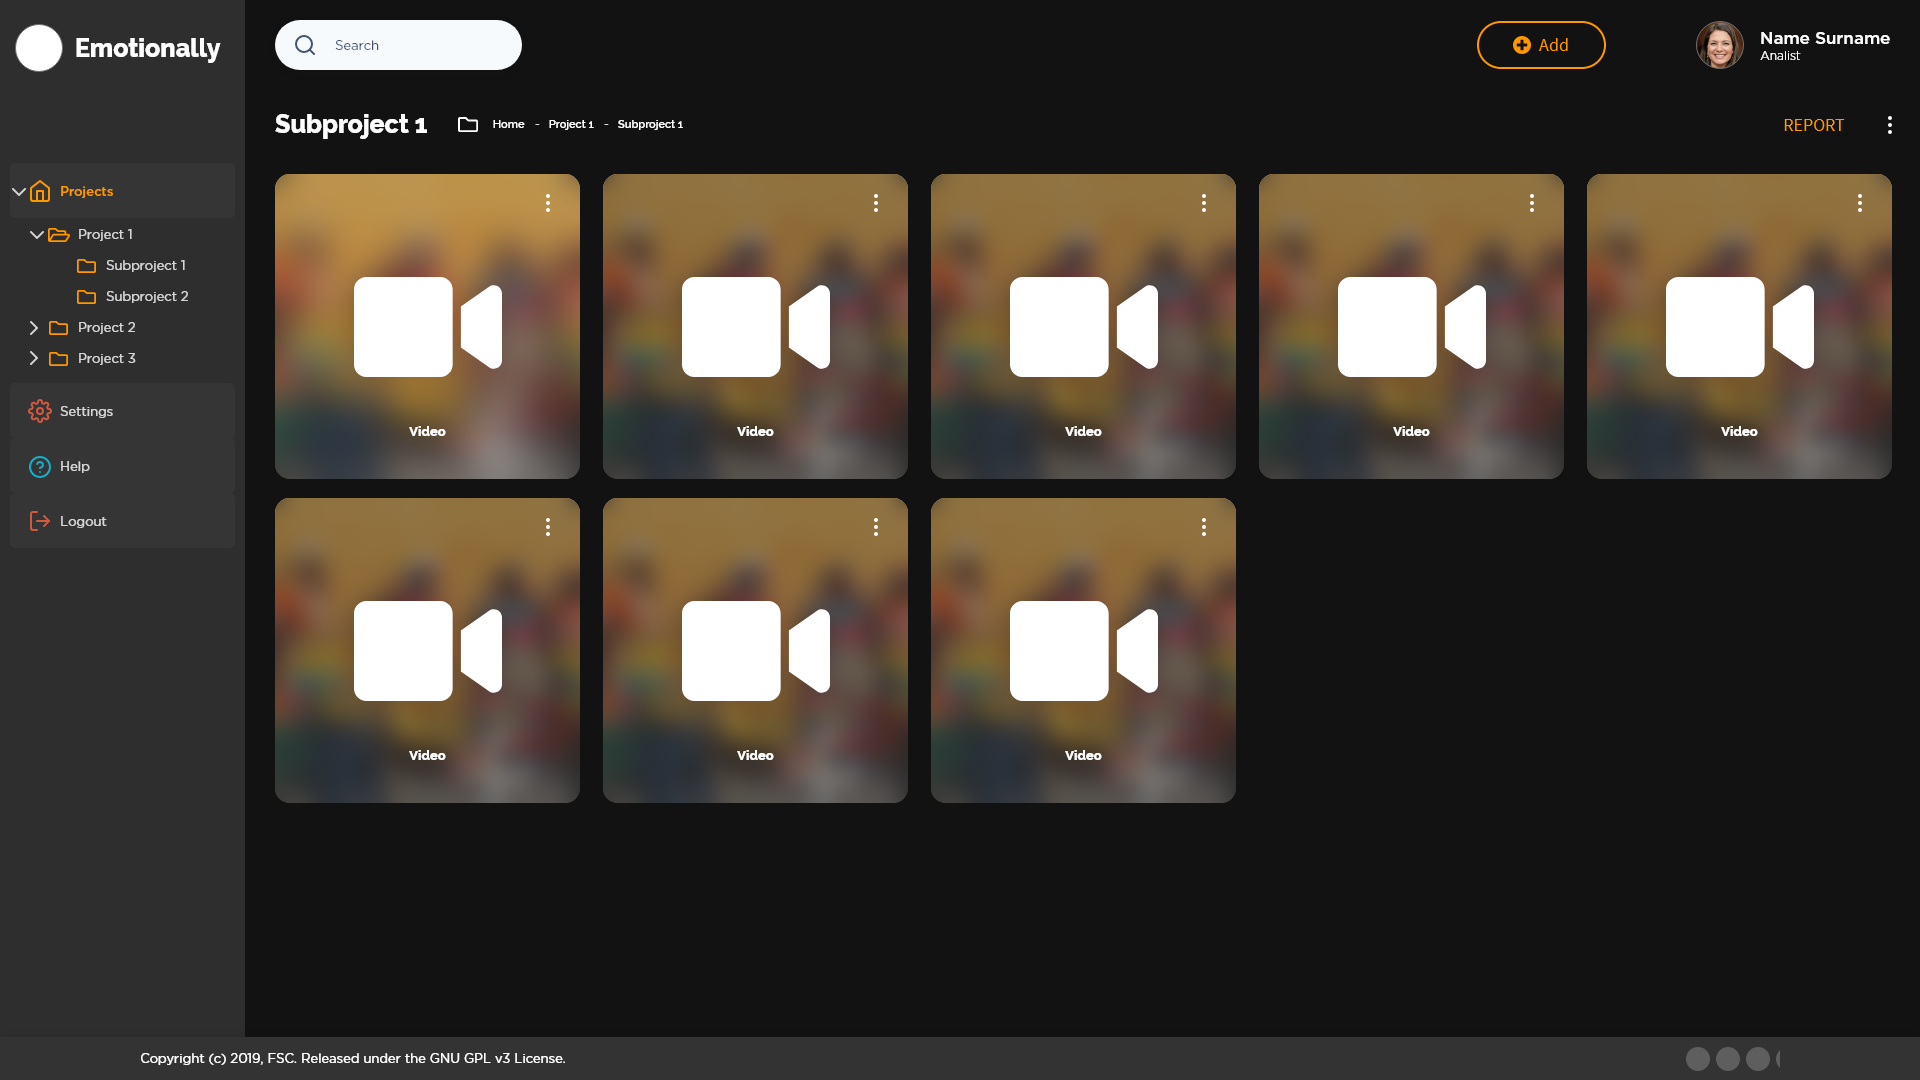
\includegraphics[width=\textwidth]{images/prototipo-comunicazione/subproject.png}
\end{figure}

\begin{figure}[H]
	\centering
	\caption{Prototipo di comunicazione: pagina di report di un video.}
	\label{fig:prototipo-comunicazione:video-report}
	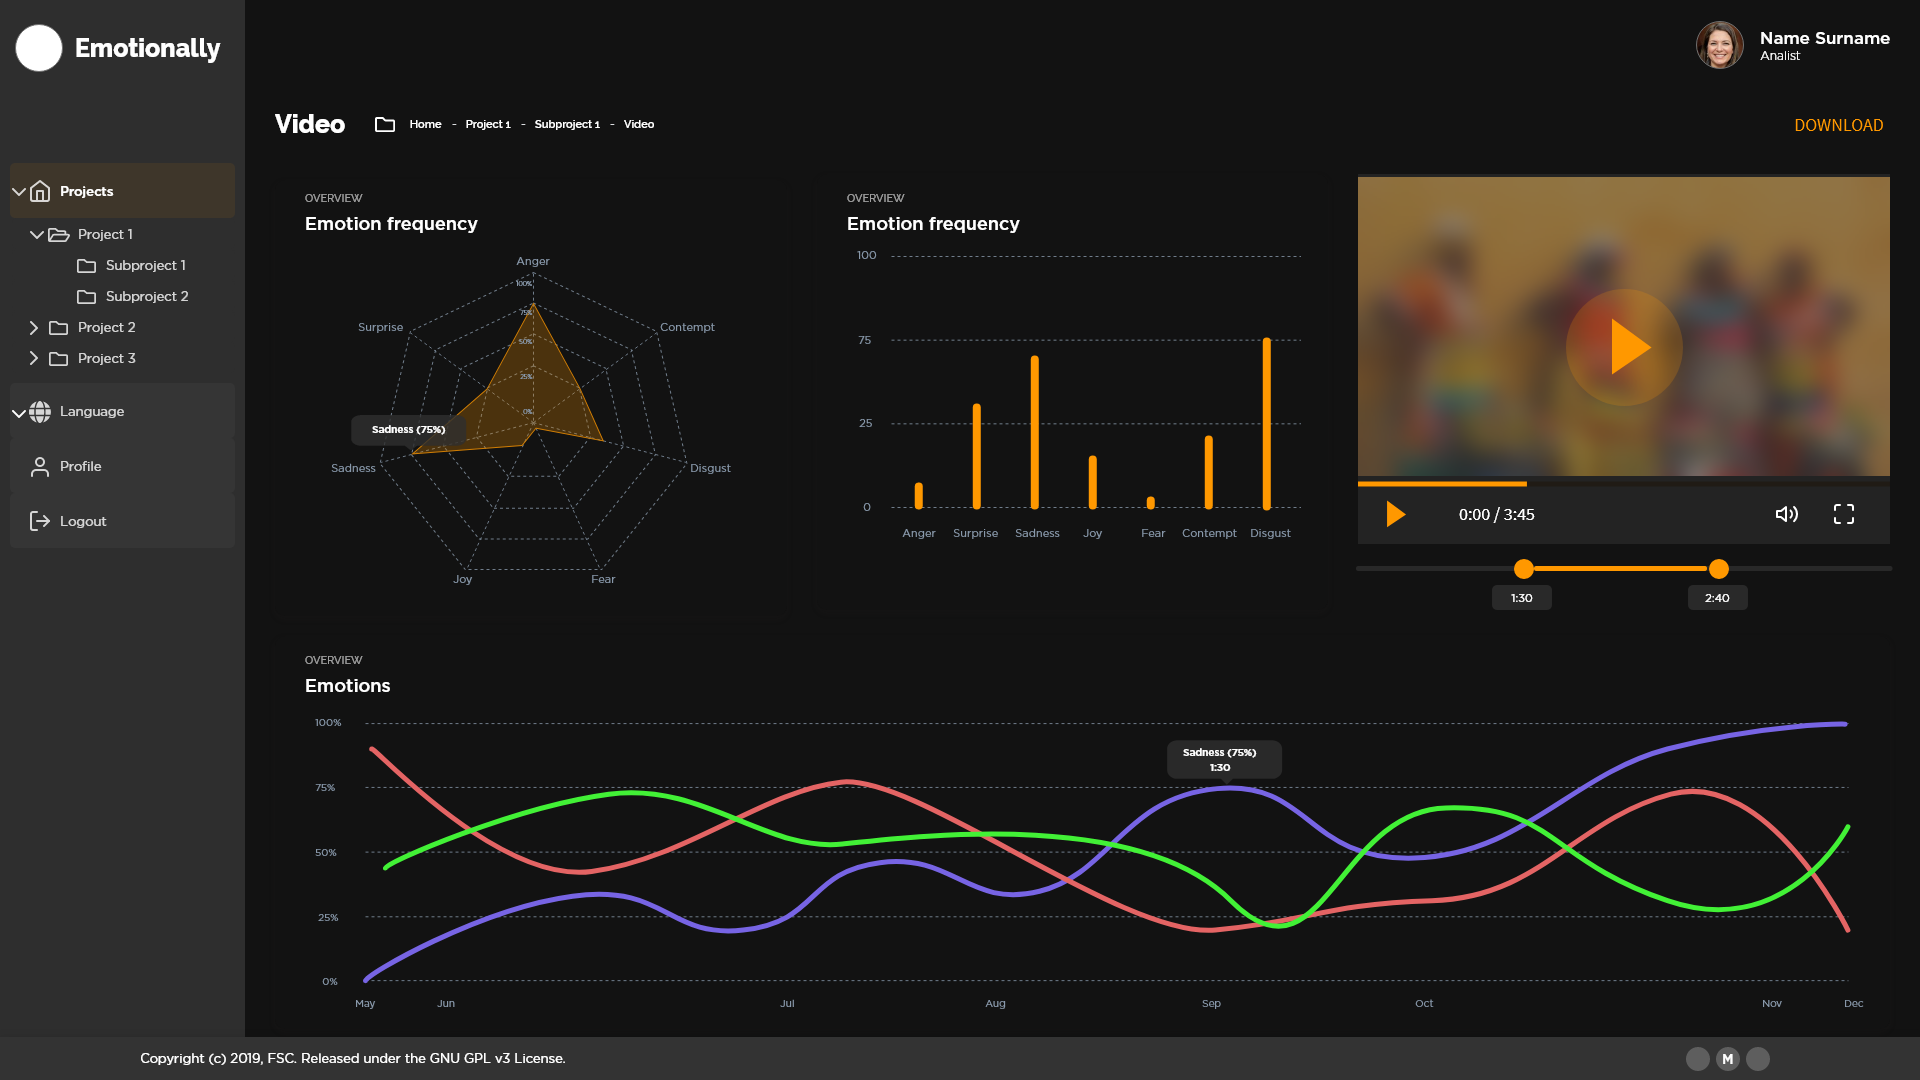
\includegraphics[width=\textwidth]{images/prototipo-comunicazione/report-video.png}
\end{figure}

\begin{figure}[H]
	\centering
	\caption{Prototipo di comunicazione: pagina di report di un progetto/sottoprogetto.}
	\label{fig:prototipo-comunicazione:project-report}
	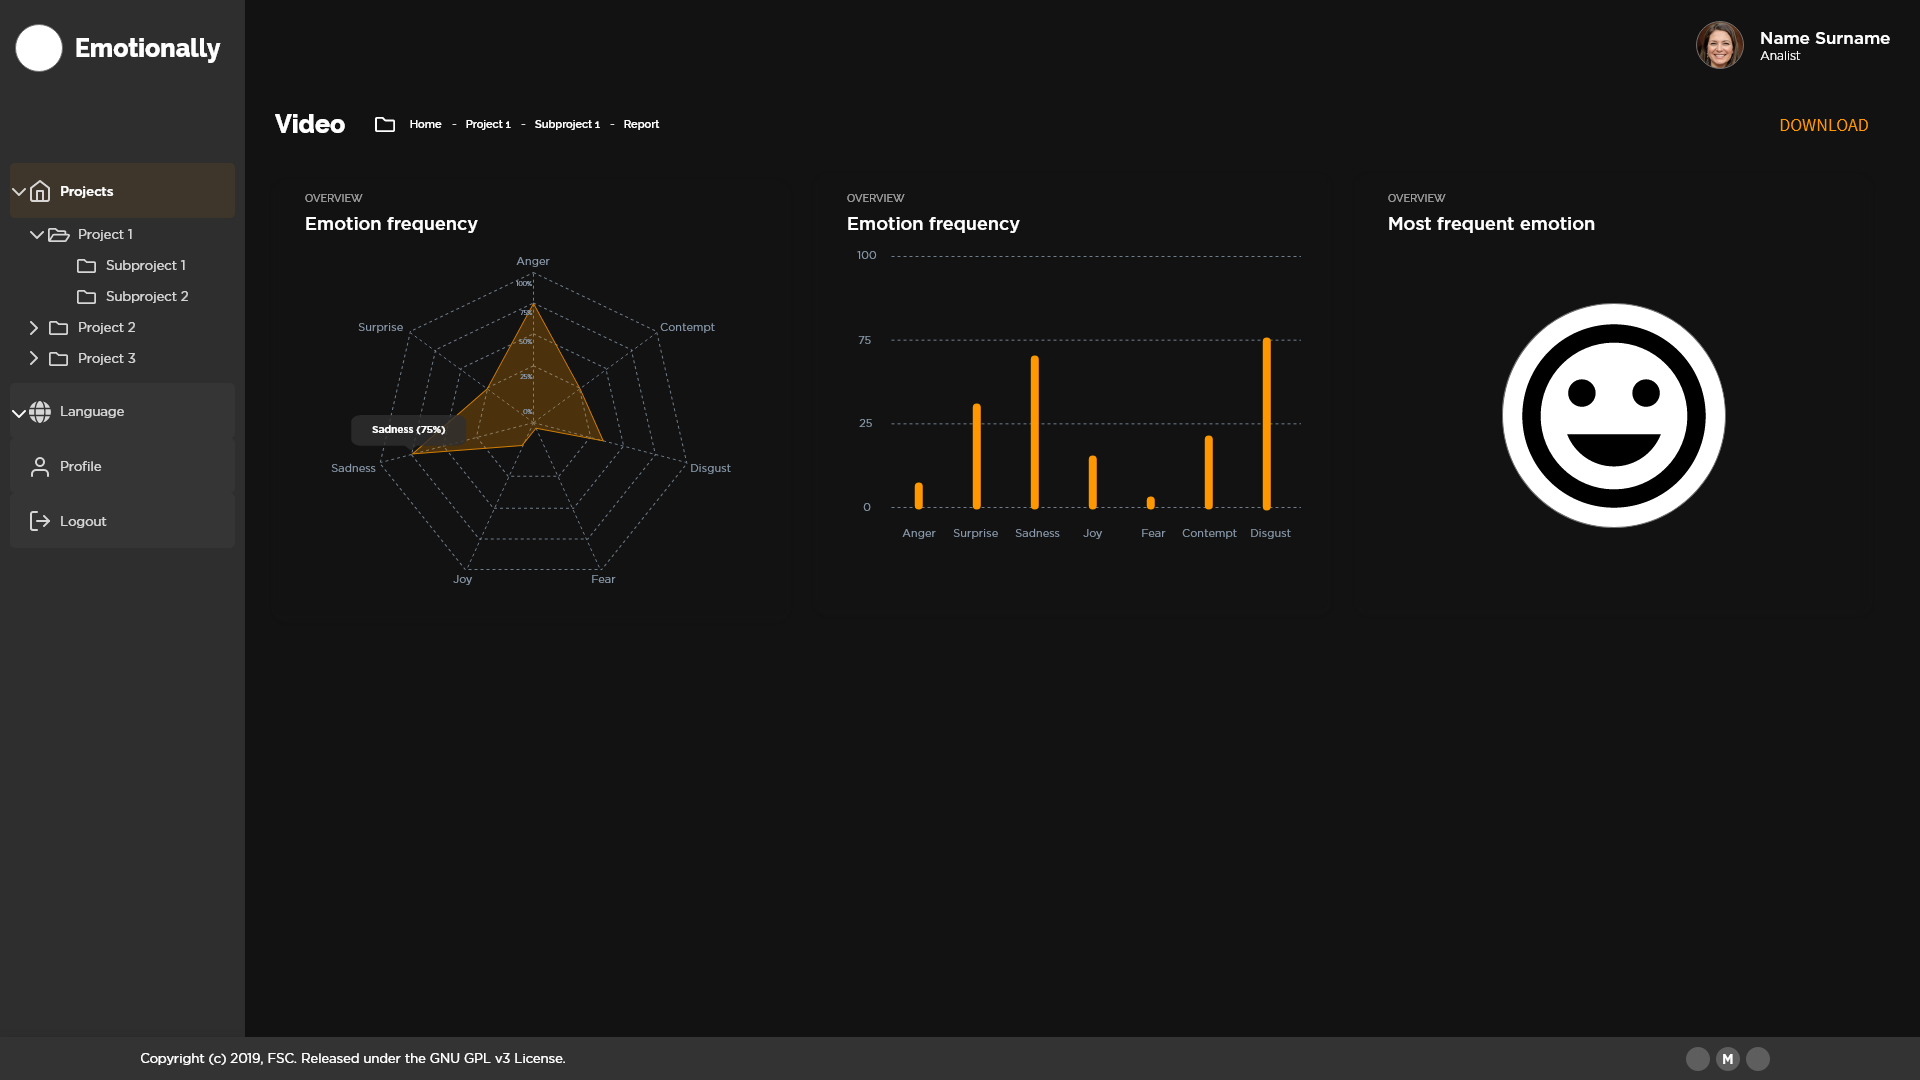
\includegraphics[width=\textwidth]{images/prototipo-comunicazione/report-project.png}
\end{figure}
